\documentclass[12pt, a4paper]{article} 
 
\usepackage[utf8]{inputenc}
 

\usepackage[bottom = 8em]{geometry} % to change the page dimensions
\geometry{a4paper} % or letterpaper (US) or a5paper or....
 
\usepackage{graphicx} % support the \includegraphics command and options
 
\usepackage{booktabs} % for much better looking tables
\usepackage{array} % for better arrays (eg matrices) in maths
\usepackage{float}
\usepackage{paralist} % very flexible & customisable lists (eg. enumerate/itemize, etc.)
\usepackage{verbatim} % adds environment for commenting out blocks of text & for better verbatim
\usepackage{subfig} % make it possible to include more than one captioned figure/table in a single float
% These packages are all incorporated in the memoir class to one degree or another...
 
 
\usepackage{float}
\usepackage{amsmath, amssymb}% for mathematical symbols
\usepackage[colorlinks=true,linkcolor=black]{hyperref} % for hyperreferences with black color
%\usepackage[T1]{fontenc} % Uncomment for norwegian document
%\usepackage[norsk]{babel} %
 
%%% HEADERS & FOOTERS
\usepackage{fancyhdr} % This should be set AFTER setting up the page geometry
\pagestyle{fancy} % options: empty , plain , fancy
\renewcommand{\headrulewidth}{0pt} % customise the layout...
\lhead{}\chead{}\rhead{}
\lfoot{}\cfoot{\thepage}\rfoot{}

 
%%% SECTION TITLE APPEARANCE
\usepackage{sectsty}
\allsectionsfont{\sffamily\mdseries\upshape} % (See the fntguide.pdf for font help)
% (This matches ConTeXt defaults)
 
%%% ToC (table of contents) APPEARANCE
\usepackage[nottoc,notlof,notlot]{tocbibind} % Put the bibliography in the ToC
\usepackage[titles,subfigure]{tocloft} % Alter the style of the Table of Contents
\renewcommand{\cftsecfont}{\rmfamily\mdseries\upshape}
\renewcommand{\cftsecpagefont}{\rmfamily\mdseries\upshape} % No bold!
 
 
%%% END Article customizations
 
%%% The "real" document content comes below...
 
\title{AI prog 3}
\author{Eivind Hærum \& \ Hong-Dang Lam}
%\date{} % Activate to display a given date or no date (if empty),
         % otherwise the current date is printed 
 
\begin{document}
\maketitle
%\begin{abstract}
% 
%Abstract
% 
%\end{abstract}
 
\newpage
\tableofcontents
\newpage
 
\section{PSO problem Task 1}
For this assignment we decided to use 100 particles, the lecturer said in a lecture that it doesn't really matter how many particle we use as long as we have more than a 10 particles.
Every particle updates their velocity vector based on this formula:
\begin{center}
$\vec{v}(t+1)=\vec{v}(t)+(c_1*r_1*(\vec{p}(t)-\vec{x}(t))) +(c_2*r_2*(\vec{g}(t)-\vec{x}(t)))$
\end{center}
Where $x$ is the current position of the particle, $p$ is the local best seen position for the particle and $g$ is the global best position seen by the social topology (either all particles or k-nearest neighbor's best known position).\\
$r_1$ and $r_2$ are random values in the range $[0,1)$ while $c_1$ and $c_2$ are weights for global/social and local attraction in the range $[0,2)$. The random values are in the formula to prevent that particle might get stuck in a knot/local maxima.\\
The position is the updated by using $\vec{x}(t+1)=\vec{x}(t)+\vec{v}(t+1)$
All the runs we do in Task 1 (b and c) are done with full social topology.
$c_1$ and $c_2$ are set to both be 0.5. These numbers do not seem to have any impact on the runs, however we decided to use 0.5 because that's what the "studass" suggested when we had problems with our code.

\subsection{Task a}
See the code provided and refer to the demonstration.
The code can be run yourself by running the main inside the runPSO.java file.


\subsection{Task b}
The global fitness is calculated by using the formula $f(\vec{(g)})=g^2$ where $g$ is the global best position seen by the topology. This means that if there's one single particle that have a position that yields a fitness less than 0.001 the code will terminate because this is considered a goal state. Our understanding of this fitness function is basically the length of the position vector squared, so if a particle have a best global position at (0.5,0.5) that means the fitness function will give us $0.5^2 + 0.5^2 = 0.5$. So whenever the best global position have a position vector length less than 0.001 it is considered a terminal state.\\
The 10 runs of the 1D circle problem is listed up the table below.
\begin{figure}[H]
\begin{center}
\begin{tabular}{l| l  c}
Run \# & Global fitness& Iterations\\ \hline
1&$2.5279044023866515*10^{-5}$ & 1 \\
2&$3.664100719971322*10^{-4}$ & 1 \\
3&$1.4212923947371634*10^{-4}$ & 1 \\
4&$7.134222602431188*10^{-4}$ & 1 \\
5&$5.494592893336489*10^{-4}$ & 1 \\
6&$7.859667993098685*10^{-4}$ & 1 \\
7&$2.3638379101551522*10^{-4}$ & 1 \\
8&$2.944787283959108*10^{-4}$ & 1 \\
9&$2.3309522255316465*10^{-4}$ & 1 \\
10&$1.4893543993401177*10^{-4}$ & 1 \\
\end{tabular}
\caption{10 runs of the 1D circle problem}
\end{center}
\end{figure}
1 iteration in this case means that the particle have already been initialized and then been "updated" once, because initializing counts as iteration number 0.

\subsection{Task c}
The run of the 2D circle problem. We decided to use 10 runs on this assignment too because we felt that 1 run only wasn't providing sufficient data. The runs can is shown on the table below.
\begin{figure}[H]
\begin{center}
\begin{tabular}{l| l  c}
Run \# & Global fitness& Iterations\\ \hline
1&$3.8168253161518443*10^{-4}$ & 175\\ 
2&$4.243457509488848*10^{-4}$ & 203\\
3&$3.9406424072396047*10^{-4}$ & 18\\ 
4&$7.435433559028153*10^{-4}$ & 30\\
5&$2.3583403176644232*10^{-5}$ & 111\\ 
6&$5.247282371692319*10^{-4}$ & 16\\ 
7&$1.1476111187016657*10^{-4}$ & 4\\ 
8&$3.595110993895342*10^{-4}$ & 139\\
9&$1.8857838445339898*10^{-4}$ & 16\\ 
10&$2.1871500510193647*10^{-4}$ & 126\\ 
\end{tabular}
\caption{10 runs of the 2D circle problem}
\end{center}
\end{figure}
As we can see in this table; it takes more iterations to find the rooster/goal for the particles than in the 1D circle problem due to the extra dimension added - this adds more search space so it takes more time for the particles to find the goal.

\section{Task 2}
This task uses k-nearest neighbor topology. The particles will only update the $\vec{g}$ based on its 3 nearest neighbor's $\vec{g}$. 
\subsection{Task a}
1D and 2D run of 3 nearest neighbor without decreasing inertia weight.

\begin{figure}[H]

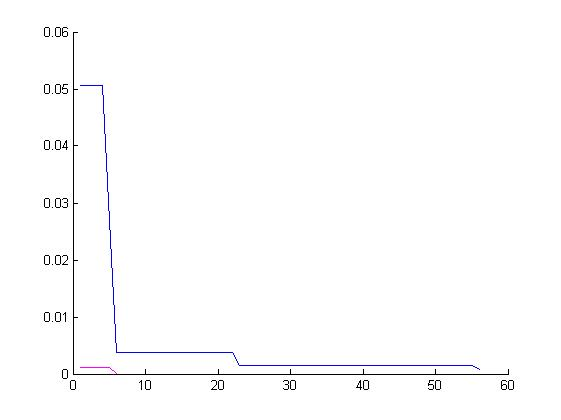
\includegraphics[width=\linewidth]{3nn_no_inertia}
\caption{runs of 1d and 2d problem with 3 nearest neighbor topology, no decreasing inertia weight\\
Magenta small line is 1d, Blue one is 2d}


\end{figure}
\subsection{Task b}
1D and 2D run of 3 nearest neighbor with decreasing inertia weight.
$\vec{v}(t+1)=(w*\vec{v}(t))+(c_1*r_1*(\vec{p}(t)-\vec{x}(t))) +(c_2*r_2*(\vec{g}(t)-\vec{x}(t)))$\\
The inertia weight $w$ decreases from 1.0 to 0.4, the decrease rate depends on the number of iterations we have decided to use. If there's 1000 iteration for a run, $w$ will decrease by $\frac{1-0.4}{1000} = 0.0006
$ for each iteration.
\begin{figure}[H]
\begin{center}
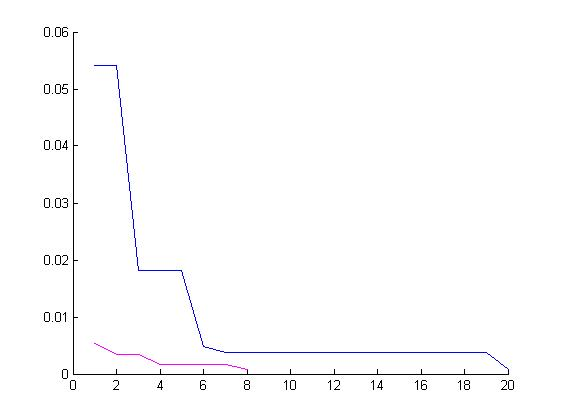
\includegraphics[width=\linewidth]{3nn_with_inertia}
\caption{runs of 1d and 2d problem with 3 nearest neighbor topology with decreasing inertia weight\\
Magenta small line is 1d, Blue one is 2d}
\end{center}

\end{figure}
\section{Task 3}\label{3}
For this task we decided to use the binary knapsack solution as suggested by the lecturer. Every particle have n dimensions (where n is number of packages) and for every dimension there's either a position 0 or 1 that shows if the package is included or not.
In other (more precise words):
For every particle there's n number of dimensions, $x_j$ can either be 0 or 1.
If $x_j = 1$ then package number $j$ is included in the container, if $x_k = 0$ then package number $k$ is not included in the container.

\subsection{Task a}
See the code provided and refer to the demonstration.
The code can be run yourself by running the main inside the runPSO.java file.

\subsection{Task b}
\begin{figure}[H]
\begin{center}
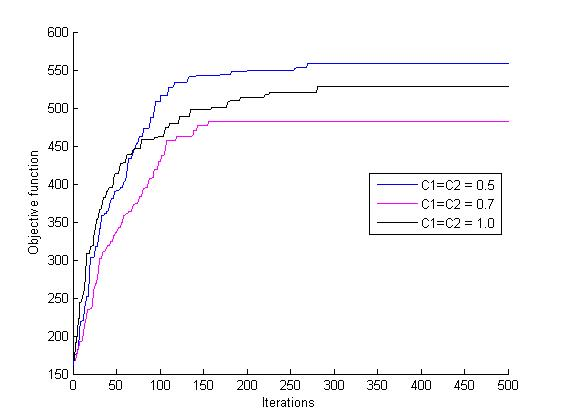
\includegraphics[width=\linewidth]{KnapSack_noInertia}
\caption{3 runs of the knapsack particle problem, 4000 particles. Graph shows global fitness}
\end{center}

\end{figure}
It's pretty interesting to see the different runs. The run where $C_1$ and $C_2$ is 0.5 seems to find a good value but the run where both values are 0.7 didn't seem to be on par with the other two runs. We think that the most important factor that might affect the end result is the initial packages chosen, but we don't know if this is actually true. The particles are supposed to "jiggle" enough to get out of a knot (or local maximum) but it might get stuck.



\subsection{Task c}
\begin{figure}[H]
\begin{center}
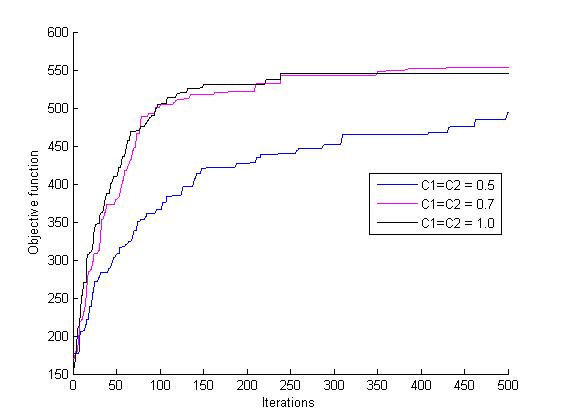
\includegraphics[width=\linewidth]{KnapSack_withInteria}
\caption{3 runs of the knapsack particle problem, 4000 particles, decreasing inertia weight. Graph shows global fitness}
\end{center}
\end{figure}

\section{Task 4}
The Knapsack PSO problem from Task \ref{3} is extended with random volume values for each package. These values range from $1m^3$ to $5m^3$, however due to a notice on It's learning we decreased the max volume from $1000m^3$ to $250m^3$.
\begin{figure}[H]
\begin{center}
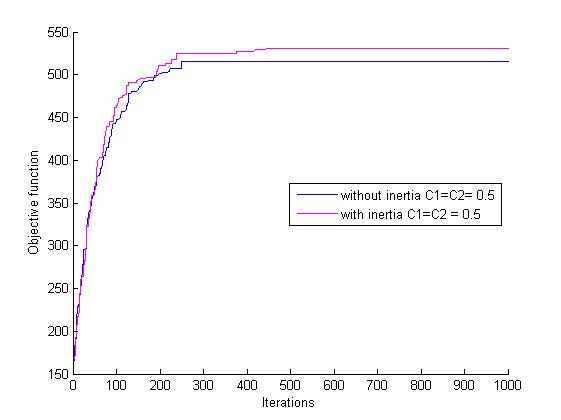
\includegraphics[width=18cm]{KnapSack_Volume}
\caption{2 runs of knapsack PSO with volume restrictions one with decreasing inertia, one with static inertia weight}
\end{center}

\end{figure}

\end{document}